\documentclass[11pt]{article}
\usepackage[margin = 1in]{geometry}
\usepackage{amsmath}
\usepackage{amssymb}
\usepackage{amsthm}
\usepackage{array}
\usepackage{multicol}
\usepackage{graphicx}
\usepackage{enumitem}
\usepackage{pdfpages}
\usepackage{url}
\usepackage[parfill]{parskip}
\usepackage{listings}
\usepackage{caption}
\usepackage{subcaption}
\usepackage[utf8]{inputenc}
% ------ Codoing Packages ------ %

\usepackage{xcolor}
\definecolor{codegreen}{rgb}{0,0.6,0}
\definecolor{codegray}{rgb}{0.5,0.5,0.5}
\definecolor{codepurple}{rgb}{0.58,0,0.82}
\definecolor{backcolour}{rgb}{0.95,0.95,0.92}
\lstdefinestyle{mystyle}{
	backgroundcolor=\color{backcolour},
	commentstyle=\color{codegreen},
	keywordstyle=\color{magenta},
	numberstyle=\tiny\color{codegray},
	stringstyle=\color{codepurple},
	basicstyle=\ttfamily\footnotesize,
	breakatwhitespace=false,
	breaklines=true,
	captionpos=b,
	keepspaces=true,
	numbers=left,
	numbersep=5pt,
	showspaces=false,
	showstringspaces=false,
	showtabs=false,
	tabsize=2
}
\lstset{style=mystyle}

% ------ Codoing Packages ------ %

\newcommand{\skipline}{\vspace{\baselineskip}}
\newcommand{\spacer}{\noalign{\medskip}}
\newcommand{~}{\sim}
\newcommand{\qrarrow}{\quad \rightarrow \quad}
\newcommand{\qqrarrow}{\qquad \rightarrow \qquad}
\newcommand{\partiald}[2]{\frac{\partial #1}{\partial #2}}
\newenvironment{problem}[1]{\textbf{Problem #1: }}{\newpage}
\newenvironment{alist}{\begin{enumerate}[label=(\alph*)]}{\end{enumerate}}
\newenvironment{rlist}{\begin{enumerate}[label=(\roman*)]}{\end{enumerate}}
\newenvironment{nlist}{\begin{enumerate}[label=(\arabic*)]}{\end{enumerate}}

\begin{document}

	\begin{center}
		\textbf{Homework 3} \\
		\textbf{Discrete Dynamical Systems and Chaos} \\
		\textbf{Math 538} \\
		\textbf{Stephen Giang RedID: 823184070} \\
		\skipline \skipline
	\end{center}

    \begin{problem}{- Plot Figures}
        See below my own plots of figures (1.6) and (1.7)
        \begin{figure}[h!]
            \centering
            \includegraphics*[width=0.5\textwidth]{figs/fig1.6-plot.png}
        \end{figure}
        \begin{figure}[h!]
            \centering
            \includegraphics*[width=1\textwidth]{figs/fig1.7-plot.png}
        \end{figure}
    \end{problem}

    \begin{problem}{T1.5}
        The map $f(x) = 2x^2 - 5x$ on $\mathbb{R}$ has fixed points at $x = 0$ and $x = 3$. Find a period-two orbit for $f$ by solving $f^2(x) = x$ for $x$.
        \\ \\
        First we should find $f^2(x)$:
        \begin{align*}
            f^2(x) = f(f(x)) &= 2(2x^2 - 5x)^2 - 5(2x^2 - 5x) \\
            &= 2(4x^4 - 20x^3 + 25x^2) - 5(2x^2 - 5x) \\
            &= 8x^4 - 40x^3 + 50x^2 -10x^2 + 25x \\
            &= 8x^4 - 40x^3 + 40x^2 + 25x
        \end{align*}
        Now we set $f^2(x) = x$ and solve for $x$ to find the period-two orbits:
        \begin{align*}
            8x^4 - 40x^3 + 40x^2 + 25x &= x \\
            8x^4 - 40x^3 + 40x^2 + 24x &= 0 \\
            8x(x^3 - 5x^2 + 5x + 3) &= 0
        \end{align*}
        Using Rational Root Theorem, and then long division, we get the following:
        \begin{align*}
            8x(x^3 - 5x^2 + 5x + 3) &= 0 \\
            8x(x-3)(x^2 - 2x - 1) &= 0
        \end{align*}
        Solving for $x$, we get the following values for $x$ that satisfy $f^2(x) = x$:
        \[x = 0, 3, 1 \pm \sqrt{2}\]
        Because, we already know that $x = 0$ and $x = 3$ are fixed points, we get period-two orbits at:
        \[x = 1 \pm \sqrt{2}\]
    \end{problem}

    \begin{problem}{T1.7}
        Find the period-two orbit of $G(x) = 4x(1 - x)$
        \\ \\
        First we should find $G^2(x)$:
        \begin{align*}
            G^2(x) = G(G(x)) &= 4(4x(1 - x))(1 - (4x(1 - x))) \\
            &= (16x - 16x^2)(1 - 4x + 4x^2) \\
            &= -64x^4 + 128x^3 - 80x^2 + 16x
        \end{align*}
        Now we set $G^2(x) = x$ and solve for $x$ to find the period-two orbits:
        \begin{align*}
            -64x^4 + 128x^3 - 80x^2 + 16x &= x \\
            -64x^4 + 128x^3 - 80x^2 + 15x &= 0 \\
            x(64x^3 - 128x^2 + 80x - 15) &= 0
        \end{align*}
        Using Rational Root Theorem, and then long division, we get the following:
        \begin{align*}
            x(64x^3 - 128x^2 + 80x - 15) &= 0 \\
            x\left(x - \frac{3}{4}\right)(4)(16x^2 - 20x + 5) &= 0
        \end{align*}
        Solving for $x$, we get the following values for $x$ that satisfy $f^2(x) = x$:
        \[x = 0, \frac{3}{4}, \frac{5 \pm \sqrt{5}}{8}\]
        Through observation, we can see that $x = 0$ and $x = 3/4$ are fixed points, thus leading us to the period-two orbits being:
        \[x = \frac{5 \pm \sqrt{5}}{8}\]
    \end{problem}

    \begin{problem}{T1.8}
        Let $G(x) = 4x(1 - x)$. Prove that for each positive integer $k$, there is an orbit of period-$k$
        \\ \\
        Notice we have found the period-one and period-two orbits, so the proof will be for $k \geq 3$:
        \\ \\
        We can see that the sum of all period points can be calculated with the following:
        \[S = 2 + \sum_{n = 2}^{k - 1} 2 ^{n-2}\]
        To prove that there exists at least one period-$k$ orbit, then we need to prove the following inequality is true:
        \begin{align*}
            2^k  - S &> k \\
            2^k - 2 - \sum_{n = 2}^{k - 1} 2 ^{n-2} &> k \\
            2^k - 2 - \sum_{n = 0}^{k - 3} 2 ^{n} &> k \\
            2^k - 2 - \frac{2^{k-3} - 1}{2 - 1} &> k \\
            2^k - 2 - (2^{k-3} - 1) &> k \\
            2^k - 1 - 2^{k-3} &> k \\
            8(2^{k - 3}) - 1 - 2^{k-3} &> k \\
            7(2^{k - 3}) - 1 &> k
        \end{align*}
        We can see that for $k \geq 3$, the left side is always greater than the right side, thus there exists at least one period-$k$ orbit for $G(x)$
        \begin{figure*}[h!]
            \centering
            \includegraphics*[width=0.5\textwidth]{figs/probt1.8.PNG}
        \end{figure*}
    \end{problem}

    \begin{problem}{T1.9}
        Let $G(x) = 4x(1 - x)$.
        \begin{alist}
            \item Decide whether the fixed points and period-two points of $G$ are
            sinks.
            \\ \\
            Noitce the following to get the fixed points`':
            \begin{align*}
                G(x) = 4x(1 - x) &= x \\
                4x - 4x^2 &= x \\
                -4x^2 + 3x &= 0 \\
                x(-4x + 3) &= 0
            \end{align*}
            From this, we get
            \[x = 0, \frac{3}{4}\]
            Now we evaluate these points at $G'(x)$ to determine stability:
            \[G'(x) = 4 - 8x \qquad |G'(0)| = |4| > 1 \qrarrow |G'(\frac{3}{4})| = |-2| > 1\]
            By Theorem 1.5, we can see that $x = 0$ and $x = \frac{3}{4}$ are both sources.
            \\ \\
            We also get the following period-two orbits from Problem T1.7 (See Page 3):
            \[x = \frac{5 \pm \sqrt{5}}{8}\]
            Now we evaluate these points at $G'(x)$ to determine stability:
            \[\left|G'\left(\frac{5 + \sqrt{5}}{8}\right)G'\left(\frac{5 - \sqrt{5}}{8}\right)\right| = |(-1 - \sqrt{5})(-1 + \sqrt{5})| = 4 > 1 \]
            By Theorem 1.5, we can see that $x = \frac{5 \pm \sqrt{5}}{8}$ are both period-two sources.
            \item Continue the periodic table for $G$ begun in Table 1.3. In particular, how many periodic orbits of (minimum) period $k$ does $G$ have, for each $k \leq 10$?
            \begin{center}
                \begin{tabular}{ | m{1.5cm} | m{2.5cm}| m{5cm} | m{3cm} |}
                 \hline
                 Period $k$ & Fixed Points of $G^k$ & Fixed Points of $G^k$ due to Lower Period Orbits & Orbits of Period $k$ \\
                 \hline\hline
                 1 & 2 & 0 & 2 \\
                 \hline
                 2 & 4 & 2 & 1 \\
                 \hline
                 3 & 8 & 2 & 2 \\
                 \hline
                 4 & 16 & 4 & 3 \\
                 \hline
                 5 & 32 & 2 & 6 \\
                 \hline
                 6 & 64 & 10 & 9 \\
                 \hline
                 7 & 128 & 2 & 18 \\
                 \hline
                 8 & 256 & 16 & 30 \\
                 \hline
                 9 & 512 & 8 & 56 \\
                 \hline
                 10 & 1024 & 34 & 99 \\
                 \hline
                \end{tabular}
            \end{center}
        \end{alist}
    \end{problem}

    \begin{problem}{1.5}
        Is the period-two orbit of the map $f(x) = 2x^2 - 5x$ on $\mathbb{R}$ a sink, a source, or neither? See Exercise T1.5.
        \\ \\
        From Exercise T1.5, we got two values for period-two orbit of the map $f(x) = 2x^2 - 5x$:
        \[x = 1 \pm \sqrt{2}, x_1 = 1 + \sqrt{2}, x_2 = 1 - \sqrt{2}, \]
        To classify this orbit as a sink or a source, we need to evaluate the value of $f^{2'}(x_1)$:
        \[f^{2'}(x) = f'(f(x_1))f'(x_1) = f'(x_2)f'(x_1)\]
        Notice the derivative of $f$ below:
        \[f'(x) = 4x - 5\]
        such that we get the following:
        \[|f'(x_2)f'(x_1)| = |f'(1 - \sqrt{2})f'(1 + \sqrt{2})| > 1 \]
        Thus by Theorem 1.5, we get that $x_1$ and $x_2$ are period-two orbit sources.
    \end{problem}

    \begin{problem}{1.7}
        Define the tent map on the unit inverval $[0, 1]$ by
        $$
        T(x) = \begin{cases}
            2x & 0 \leq x \leq 1/2 \\
            2(1 - x) & 1/2 \leq x \leq 1 \\
        \end{cases}
        $$
        \begin{alist}
            \item Divide the unit interval into two appropriate subintervals and repeat parts (a) - (c) of Exercise 1.6 for this map.
            \begin{figure}[h!]
                \centering
                \includegraphics*[width=0.55\textwidth]{figs/prob1.7a.PNG}
            \end{figure}
            \begin{figure}[h!]
                \centering
                \includegraphics*[width=0.55\textwidth]{figs/prob1.7a2.PNG}
            \end{figure}
            \\
            Notice that because the shape of the graph are linear, we know that at half the $x$ interval, it maps to half $f$ interval.  Such that each interval will be exactly half of the previous.  The 2nd iterate will be at a quarter of the distance.
            \newpage
            \item Complete a periodic table for $f$, similar to the one in Table 1.3, for periods less than or equal to 10. In what ways, if any, does it differ from the periodic table for the logistic map $G$?
            \begin{center}
                \begin{tabular}{ | m{1.5cm} | m{2.5cm}| m{5cm} | m{3cm} |}
                 \hline
                 Period $k$ & Fixed Points of $T^k$ & Fixed Points of $T^k$ due to Lower Period Orbits & Orbits of Period $k$ \\
                 \hline\hline
                 1 & 2 & 0 & 2 \\
                 \hline
                 2 & 2 & 2 & 0 \\
                 \hline
                 3 & 2 & 2 & 0 \\
                 \hline
                 4 & 2 & 2 & 0 \\
                 \hline
                 5 & 2 & 2 & 0 \\
                 \hline
                 6 & 2 & 2 & 0 \\
                 \hline
                 7 & 2 & 2 & 0 \\
                 \hline
                 8 & 2 & 2 & 0 \\
                 \hline
                 9 & 2 & 2 & 0 \\
                 \hline
                 10 & 2 & 2 & 0 \\
                 \hline
                \end{tabular}
            \end{center}
        \end{alist}
    \end{problem}

    \begin{problem}{1.10}
        For the map $g(x) = 3.05x(1 - x)$, find the stability of all fixed points and period-two points.
        \\ \\
        To find all the fixed points, we need to solve $f(x) = x$ for $x$:
        \begin{align*}
            f(x) = 3.05x(1 - x) &= x \\
            3.05x - 3.05x^2 &= x \\
            2.05x - 3.05x^2 &= 0 \\
            x(2.05 - 3.05x) &= 0
        \end{align*}
        From here, we get the following fixed points:
        \[x = 0, \frac{2.05}{3.05}\]
        To find its stability, we now need to evaluate $|f'(x)|$ at these values:
        \[|f'(x)| = |3.05 - 6.10x| \qqrarrow |f'(0)| = |3.05| > 1 \qquad |f'(\frac{2.05}{3.05})| = |-1.05| > 1\]
        Thus, we get that the following fixed points are both sources:
        \[x = 0, \frac{2.05}{3.05}\]
        To find period-two orbits, we need to solve $f^2(x) = x$ for $x$:
        \begin{align*}
            f^2(x) = 3.05(3.05x - 3.05x^2)(1 - (3.05x - 3.05x^2)) &= x \\
            (9.3025x - 9.3025x^2)(1 - 3.05x + 3.05x^2) &= x \\
            -28.372625x^4 + 56.74525x^3 - 37.675125x^2 + 9.3025x &= x \\
            -28.372625x^4 + 56.74525x^3 - 37.675125x^2 + 8.3025x &= 0 \\
            x(28.372625x^3 - 56.74525x^2 + 37.675125x - 8.3025) &= 0 \\
            x(x - \frac{2.05}{3.05})(28.372625x^2 - 37.675125x + 12.3525) &= 0
        \end{align*}
        From here, we get the following period-two orbits:
        \[x = 0, \frac{2.05}{3.05}, 0.590164, 0.737705\]
        Notice the derivative of $f$ below:
        \[f'(x) = 3.05 - 6.10x\]
        To find its stability, we now need to evaluate $|f^{2'}(x)|$ at these values:
        \[|f^{2'}(0.590164)| = |f'(0.737705)f'(0.590164)| < 1\]
        Thus, we get that the following period-two orbits are both sinks:
        \[x = 0.590164, 0.737705\]
    \end{problem}

    \begin{problem}{1.12}
        The map $g(x) = 2x(1 - x)$ has negative values for large $x$. Population biologists sometimes prefer maps that are positive for positive $x$.
        \begin{alist}
            \item  Find out for what value of $a$ the map $h(x) = axe^{-x}$ has a superstable fixed point $x_0$, which means that $h(x_0) = x_0$ and $h'(x_0) = 0$.
            \\ \\
            Firstly, notice the following:
            \[h(x_0) = ax_0e^{-x_0} \qquad \qquad h'(x_0) = -ax_0e^{-x_0} + ae^{-x_0}\]
            Now, we just use some algebra to find $x_0$:
            \begin{align*}
                h(x_0) = ax_0e^{-x_0} &= x_0 & h'(x_0) = -ax_0e^{-x_0} + ae^{-x_0} &= 0 \\
                ax_0e^{-x_0} - x_0 &= 0 & ax_0e^{-x_0} &= ae^{-x_0} \\
                x_0(ae^{-x_0} - 1) &= 0 & x_0 &= 1
            \end{align*}
            Solving the second factor of $h(x_0)$, we get:
            \[ae^{-x_0} = 1 \qqrarrow e^{-x_0} = \frac{1}{a} \qqrarrow x_0 = -\ln \frac{1}{a} = \ln a\]
            Because both conditions have to be true, we get the following equality:
            \[x_0 = \ln a = 1\]
            Thus, we get a superstable fixed point, when:
            \[a = e\]
            \item Investigate the orbit starting at $x_0 = 0.1$ for this value of $a$ using a calculator. How does the behavior of this orbit differ if $a$ is increased by 50\%?
            \\ \\
            At $x_0 = 0.1$, we see that the cobweb plot is going towards a sink at $x = 0$. But when we increase $a$ by 50\%, we got that the cobweb plot is going away from a source at $x = 0$
            \begin{figure}[h!]
                \centering
                \includegraphics*[width=0.45\textwidth]{figs/prob1.12b1.png}
                \includegraphics*[width=0.45\textwidth]{figs/prob1.12b2.png}
            \end{figure}
            \newpage
            \item What is the range of $a \geq 1$ for which $h(x)$ has a positive sink?
            \\ \\
            Notice, we only have fixed points at the following $x_0$ values:
            \[x_0 = 0 \qquad \text{ and } \qquad x_0 = \ln a\]
            Now, to get a sink, we need the following equality:
            \[h'(x) = -ae^{-x}(x - 1)\]
            Subbing in our value for $x_0$, we get:
            \[h'(x_0) = -ae^{-\ln a}(\ln a - 1) = -(\ln a - 1) = 1 - \ln a\]
            Now to get a positive sink, we solve the following inequality
            \begin{align*}
                |h'(x_0)| &< 1 \\
                -1 < 1 - \ln a &< 1 \\
                -2 < - \ln a &< 0 \\
                2 > \ln a &> 0 \\
                e^2 > a &> 1
            \end{align*}
            Thus the range for $a \geq 1$ for which $h(x)$ has a positive sink is:
            \[1 \leq a < e^2\]
        \end{alist}
    \end{problem}

    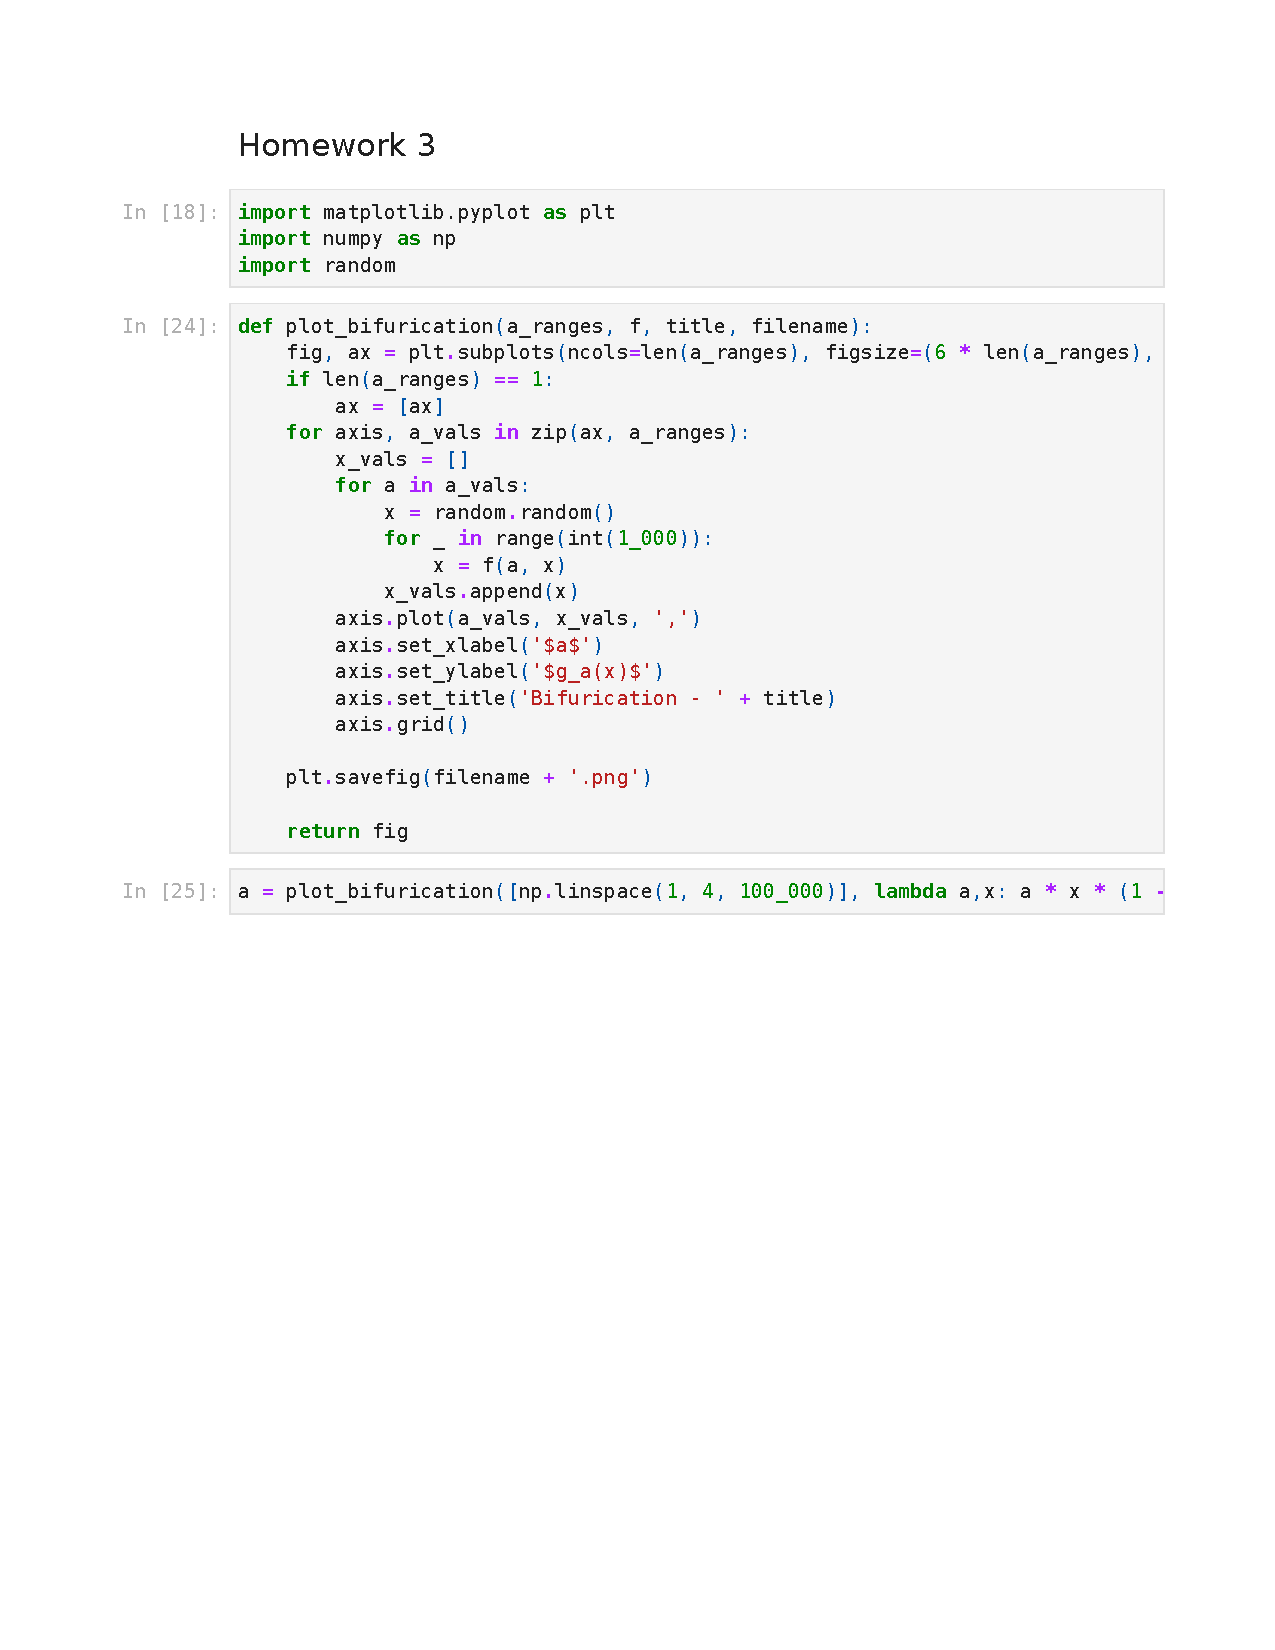
\includepdf[pages=-]{code.pdf}

\end{document}